% Drawing 69/01-10 -- folder 69, batch 01, archive page 11 (PDF page 12).
% Transcription: les graphes $D_i$ : $D_1$ le point $u$ ; $D_2$ l'arête $u v$ ; $D_3$ le triangle $u, v, w$ ; $D_4$ le triangle $u, v, w$ avec une arête pendante $u u'$ ; $D_5$ le triangle $u, v, w$ et, au-dessous, $u'$, $v'$ (la moitié inférieure d'un rectangle hachurée, reprise) ; $D_6$ un prisme triangulaire à bases $u, v, w$ et $u', v', w'$ ; $D_7$ deux prismes accolés par une face, avec les sommets $u, v, w, u', v', w', w''$ et $w'''$, dessin repris sur une première esquisse hachurée
% Kind: column of graphs D_0 ... D_7. Method 2 (schematic redraw from the facsimile). Status: partial.
% Notes: D_0 = emptyset; D_1 (circled) the point u; D_2 the edge u v (dots at both ends); D_3 (circled) the triangle u v w (dots at u, v); D_4 the triangle with the pendant edge u u'; D_5 the triangle u v w standing on a rectangle u v v' u' (top and bottom edges inked heavier), the left side of the triangle starting a little below u, the lower half of the rectangle hatched; D_6 a triangular prism u' v' w' over u, v, with w behind (the edges w' w and w v drawn as on the page; the hidden edge w u is not drawn); D_7 (circled) two prisms glued along a face. The inclusion arcs on the left are drawn as small arches. Vertices are placed once and every edge runs between them. Still differs from the facsimile: D_7 is drawn over a first, heavily inked sketch, given only by its main strokes; its letters are placed where legible (u, v, u', v', w, w', w''; w''' of the transcription is not located). A first 'D_6 =' to the left of D_7, scribbled over, is struck and not drawn. In D_5 two further letters by the top corners (reprise) are left out. Redrawn 2026-11-09 (issue 128): vertices placed once and every edge drawn between them, labels at \small, strike-outs not drawn; to check again. Question settled by a machine pass on the facsimile, 2026-11-12 (maths): each D_{i+1} adds one vertex to D_i (D_6, the triangular prism, has the six vertices u, v, w, u', v', w'), so D_7 has seven vertices and the seventh is w''; a letter w''' is not expected and none is drawn. Which edges join w'' to the prism in the overdrawn sketch of D_7 stays open (kept question). Not checked by a reader.
% Coordinates: 1 unit = 1 mm = 1/100 of the crop width (bbox in page fractions: [0.12, 0.1, 0.36, 0.44]).
% Redrawn by Claude (claude-opus-5-5), issue #73, 2026-11-09; not checked by a human; not compiled (no TeX in the session).
% Rights: reproduces part of the work -- behind RENDER_TRANSCRIPTS, never published by itself.
\documentclass[tikz,border=3pt]{standalone}
\usepackage{amsmath,amssymb}
\usetikzlibrary{patterns,arrows.meta}
\tikzset{pencil/.style={black!45}, struck/.style={black!35}, mark/.style={circle,draw,inner sep=1.3pt}, pt/.style={circle,fill,inner sep=0.9pt}, opt/.style={circle,draw,fill=white,inner sep=1.1pt}}
\begin{document}
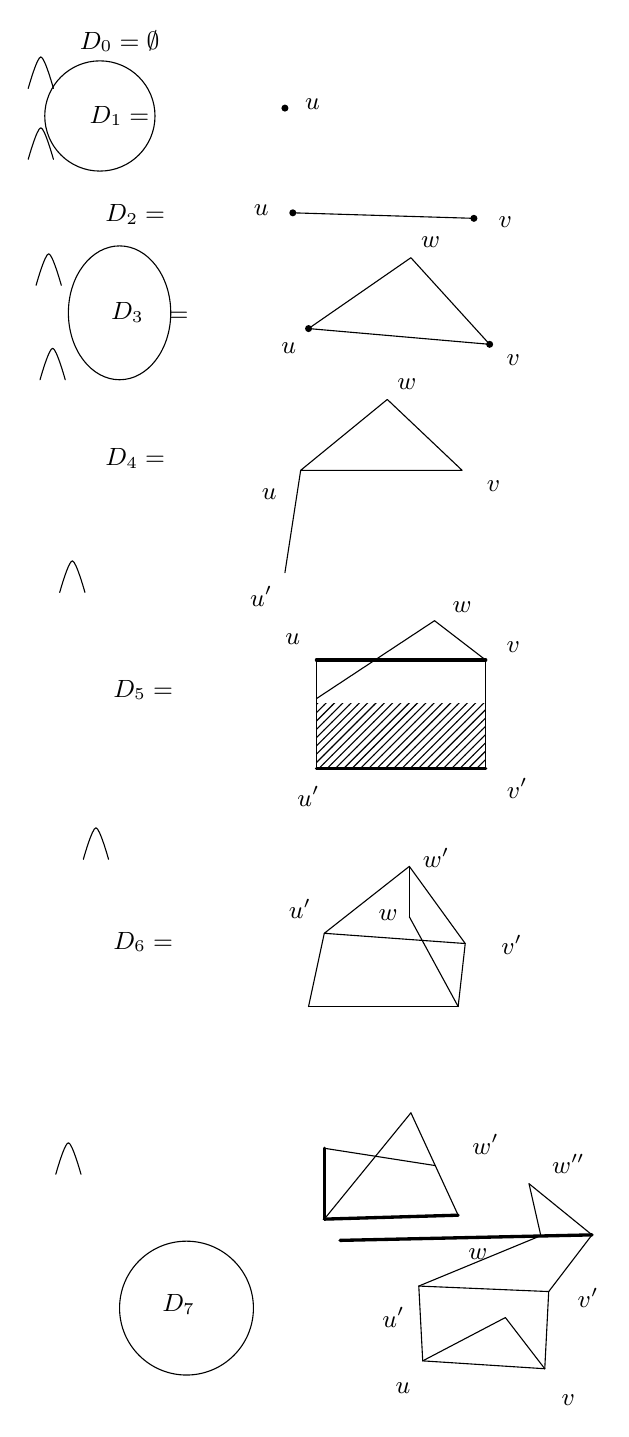
\begin{tikzpicture}[x=1mm,y=1mm,line cap=round,line join=round,font=\scriptsize]
\node[inner sep=1pt] at (34,-13.7) {\small $D_0 = \emptyset$};
\draw plot[smooth, tension=0.55] coordinates {(22.4,-19.7) (24,-15.7) (25.6,-19.7)};
\draw plot[smooth, tension=0.55] coordinates {(22.4,-28.7) (24,-24.7) (25.6,-28.7)};
\draw plot[smooth, tension=0.55] coordinates {(23.4,-44.7) (25,-40.7) (26.6,-44.7)};
\draw plot[smooth, tension=0.55] coordinates {(23.9,-56.7) (25.5,-52.7) (27.1,-56.7)};
\draw plot[smooth, tension=0.55] coordinates {(26.4,-83.7) (28,-79.7) (29.6,-83.7)};
\draw (31.5,-23.2) circle[radius=7];
\node[inner sep=1pt] at (34,-23.2) {\small $D_1 =$};
\node[pt] at (55,-22.2) {};
\node[inner sep=1pt] at (58.5,-21.7) {\small $u$};
\node[inner sep=1pt] at (36,-35.7) {\small $D_2 =$};
\draw (56,-35.5) -- (79,-36.2);
\node[pt] at (56,-35.5) {};
\node[pt] at (79,-36.2) {};
\node[inner sep=1pt] at (52,-35.2) {\small $u$};
\node[inner sep=1pt] at (83,-36.7) {\small $v$};
\draw (34,-48.2) ellipse[x radius=6.5, y radius=8.5];
\node[inner sep=1pt] at (35,-48.2) {\small $D_3$};
\node[inner sep=1pt] at (41.5,-48.7) {\small $=$};
\draw (58,-50.2) -- (81,-52.2) -- (71,-41.2) -- cycle;
\node[pt] at (58,-50.2) {};
\node[pt] at (81,-52.2) {};
\node[inner sep=1pt] at (55.5,-52.7) {\small $u$};
\node[inner sep=1pt] at (84,-54.2) {\small $v$};
\node[inner sep=1pt] at (73.5,-39.2) {\small $w$};
\node[inner sep=1pt] at (36,-66.7) {\small $D_4 =$};
\draw (57,-68.2) -- (77.5,-68.2) -- (68,-59.2) -- cycle;
\draw (57,-68.2) -- (55,-81.2);
\node[inner sep=1pt] at (53,-71.2) {\small $u$};
\node[inner sep=1pt] at (81.5,-70.2) {\small $v$};
\node[inner sep=1pt] at (70.5,-57.2) {\small $w$};
\node[inner sep=1pt] at (52,-84.2) {\small $u'$};
\node[inner sep=1pt] at (37,-96.1) {\small $D_5 =$};
\draw[very thick] (59,-92.3) -- (80.5,-92.3);
\draw (59,-92.3) -- (59,-106.1);
\draw (80.5,-92.3) -- (80.5,-106.1);
\draw[very thick] (59,-106.1) -- (80.5,-106.1);
\draw (59,-97.2) -- (74,-87.3) -- (80.5,-92.3);
\fill[pattern=north east lines] (59,-97.8) -- (80.5,-97.8) -- (80.5,-106.1) -- (59,-106.1) -- cycle;
\node[inner sep=1pt] at (56,-89.6) {\small $u$};
\node[inner sep=1pt] at (84,-90.6) {\small $v$};
\node[inner sep=1pt] at (77.5,-85.6) {\small $w$};
\node[inner sep=1pt] at (58,-109.6) {\small $u'$};
\node[inner sep=1pt] at (84.5,-108.6) {\small $v'$};
\draw plot[smooth, tension=0.55] coordinates {(29.4,-117.6) (31,-113.6) (32.6,-117.6)};
\node[inner sep=1pt] at (37,-128.1) {\small $D_6 =$};
\draw plot[smooth, tension=0.55] coordinates {(25.9,-157.6) (27.5,-153.6) (29.1,-157.6)};
\draw (42.5,-174.6) circle[radius=8.5];
\node[inner sep=1pt] at (41.5,-174.1) {\small $D_7$};
\draw (60,-127) -- (77.9,-128.3) -- (70.8,-118.5) -- cycle;
\draw (70.8,-118.5) -- (70.8,-124.9);
\draw (70.8,-124.9) -- (77,-136.3);
\draw (60,-127) -- (58,-136.3);
\draw (77.9,-128.3) -- (77,-136.3);
\draw (58,-136.3) -- (77,-136.3);
\node[inner sep=1pt] at (56.9,-123.9) {\small $u'$};
\node[inner sep=1pt] at (83.8,-128.5) {\small $v'$};
\node[inner sep=1pt] at (74.2,-117.4) {\small $w'$};
\node[inner sep=1pt] at (68.1,-124.7) {\small $w$};
\draw[very thick] (60,-154.3) -- (60,-163.3);
\draw (60,-154.3) -- (74.1,-156.5);
\draw (71,-149.8) -- (77,-162.8);
\draw (71,-149.8) -- (60,-163.3);
\draw[very thick] (60,-163.3) -- (77,-162.8);
\draw[very thick] (62,-166) -- (94,-165.3);
\draw (72,-171.8) -- (88.5,-172.5);
\draw (72,-171.8) -- (72.5,-181.3);
\draw (72.5,-181.3) -- (88,-182.3);
\draw (88.5,-172.5) -- (88,-182.3);
\draw (88.5,-172.5) -- (94,-165.3);
\draw (94,-165.3) -- (86,-158.8);
\draw (86,-158.8) -- (87.5,-165.4);
\draw (72,-171.8) -- (87.5,-165.4);
\draw (72.5,-181.3) -- (83,-175.8);
\draw (83,-175.8) -- (88,-182.3);
\node[inner sep=1pt] at (70,-184.8) {\small $u$};
\node[inner sep=1pt] at (91,-186.3) {\small $v$};
\node[inner sep=1pt] at (68.8,-175.8) {\small $u'$};
\node[inner sep=1pt] at (93.5,-173.3) {\small $v'$};
\node[inner sep=1pt] at (91,-156.3) {\small $w''$};
\node[inner sep=1pt] at (79.5,-167.8) {\small $w$};
\node[inner sep=1pt] at (80.5,-153.8) {\small $w'$};
\end{tikzpicture}
\end{document}
